\documentclass[hidelinks,11pt,titlepage,a4paper]{article} %padrao letterpaper, 10pt

% ----------------------------------------------
%Letra parecida com Arial
\usepackage{helvet}
\renewcommand{\familydefault}{\sfdefault}
\usepackage[T1]{fontenc}
% ---------------------------------------------


\usepackage[utf8]{inputenc}
\usepackage[portuguese]{babel}
\usepackage{amsfonts,amssymb,graphicx}
\usepackage[centertags]{amsmath}
\usepackage[hmargin=2.5cm,vmargin=2cm,bmargin=3cm]{geometry}
\usepackage{fancyvrb}
\usepackage{graphicx}
\usepackage{eso-pic} % marca de água para logos
\usepackage{indentfirst}
\usepackage{mathtools}
\usepackage{caption}
\usepackage{cite}
\usepackage{url}
% clever reff %
\usepackage{hyperref}
\usepackage{amsmath}


\usepackage{eqparbox,array}
\usepackage{algorithm}
\usepackage[noend]{algpseudocode}

\makeatletter
\renewcommand{\ALG@name}{Algoritmo}
\renewcommand{\listalgorithmname}{Lista de \ALG@name s}
\makeatother

\usepackage{pdflscape}

\usepackage{cleveref}
% ----------- %

% ----------------------------------------------
\usepackage{booktabs}
% Tabelas fancy
% ----------------------------------------------

% ----------------------------------------------
%gráficos fancy
\usepackage{pgfplots}
%?
\usepackage{pgfplotstable}
% ----------------------------------------------

\usepackage{minted}
\usemintedstyle{emacs}
\setminted{
frame=lines,
framesep=2mm,
baselinestretch=1.2,
fontsize=\footnotesize,
%linenos, 
breaklines,
breakautoindent=false,
autogobble
}

%%%%%%%%%%%%  CABEÇALHO  %%%%%%%%%%%%%

\usepackage{fancyhdr}
\pagestyle{fancy}
\lhead{
\includegraphics[height=0.53in]{resources/template/logo-ee.png}}
\rhead{\textsl{\leftmark}}
\cfoot{\thepage}
\renewcommand{\headrulewidth}{2pt}
\renewcommand{\footrulewidth}{1pt}

%%%%%%%%%%%%%%%%%%%%%%%%%%%%%%%%%%%%%%




%Usado em conjunto com o comando \layout. Este último mostra todos os valores
%dos elementos de página.
%\usepackage{layout}

%Mostra um conjunto de quadros/frames em cada página, correspondente ao tamanho
%de cada elemento de página, como rodapé, cabeçalho, intervalos entre estes,
%margem para notas
%
%\usepackage{showframe}

%Ajusta cabeçalho para altura do logotipo
\headheight= 44pt
%Coloca margem de notas dentro da página
\marginparwidth= 40pt


%%%%%%%%%%%%%%%%%%%%%%%%%%%%%%%%%%%%%%%%%%%%%%%%%%%%%%%%%%%%%%%%%%%%%%
%%USADO EM CONJUNTO COM O PACOTE LAYOUT
%%MOSTRA ELEMENTOS DA PÁGINA, COMO CABEÇALHO, RODAPÉ, MARGEM PARA NOTAS, CORPO
%%SEPARADORES ENTRE ELEMENTOS.
%%
%%
%\begin{figure}[htbp] 
%	\begin{center} \leavevmode 
%		\layout
%		\vspace{3cm}
%		\caption{Elementos da página. Os valores mostrados são aqueles que estão
%aplicados ao presente documento, não os valores por defeito } 
%\label{fig:layout} 
%	\end{center} 
%\end{figure}
%%%%%%%%%%%%%%%%%%%%%%%%%%%%%%%%%%%%%%%%%%%%%%%%%%%%%%%%%%%%%%%%%%%%%%%%

%--- Quotes ---%
%\usepackage{epigraph}
 
%\setlength\epigraphwidth{12cm} % default 8
%\setlength\epigraphrule{0pt}

%\begin{quote}
%	
%\end{quote}

\setcounter{secnumdepth}{4}
\setcounter{tocdepth}{4}
\setlength{\parindent}{2em}
\setlength{\parskip}{1em}
\renewcommand{\baselinestretch}{1.2}


%--- Custom Appendice ---%
%\usepackage[titletoc,toc,title]{appendix}

\pgfplotsset{compat=1.13} 



%--- Custom Appendice ---%
%\usepackage[titletoc,toc,title]{appendix}

\pgfplotsset{compat=1.13} 




\hypersetup{
pdftitle={Trabalho 1},
pdfauthor={Bruno Pereira},
%pdfsubject={Investigação Operacional},
%pdfkeywords={keyword1, keyword2}},
bookmarksnumbered=true,     
bookmarksopen=true,         
bookmarksopenlevel=1,       
colorlinks=true,            
pdfstartview=Fit,           
pdfpagemode=UseOutlines, % this is the option you were lookin for
pdfpagelayout=TwoPageRight
		}



\newenvironment{longlisting}{\captionsetup{type=listing}}{}
\begin{document}

%%%%%%%%%%%%%%%%%%%%%%%%%%%%%%%%%%%%%%%%%%%%

% ----------- %
\begin{titlepage}


\begin{minipage}{0.3\textwidth}
\begin{flushleft} 

\includegraphics[width=1.1\textwidth]{resources/template/logo-ee.png}
\end{flushleft}
\end{minipage}
\hfill
\begin{minipage}{0.6\textwidth}
\begin{flushright} 

\fontfamily{pag}\selectfont{\large \textsc{Universidade do Minho}\\[0.1cm]
\large \bfseries Mestrado Integrado em Engenharia Informática \\ [0.1cm]
\large \bfseries \textit{Computação Gráfica}\\[4mm]
}
\end{flushright}
\end{minipage}\\[1cm]


\vspace{3cm}


\begin{center}

\fontfamily{pag}\selectfont{\textsc{\Huge Trabalho Prático: 4º Fase}\\[1cm]


{\large \bfseries \Large\emph{Coordenadas de texturas e vetores normais} \\[2cm] }



\vspace{3cm}

\begin{minipage}{0.7\textwidth}
\begin{flushright} \large
\textbf{Grupo 3:}\par
	Bruno Pereira  --- 72628	
\end{flushright}
\end{minipage}


\vfill

\emph{\large Braga, {\large \today}}
}
\end{center}

\end{titlepage}

% ----------- %
\tableofcontents
\newpage
\listoffigures
\newpage
\listofalgorithms
\newpage
% ----------- %



%---------------------------------------------------------------------------------------------------------------%
\section*{Introdução\markboth{\MakeUppercase{Introdução}}{}}
\addcontentsline{toc}{section}{Introdução}
\label{intro}


Para esta fase deste projeto é requerido que se implementem texturas, luzes
e componentes de cor da luz e da reflexão da luz nos materiais, ou componentes
virtuais da reflexão do mundo real.

Pede-se que se calcule vetores normais às superfícies de todas as geometrias
criadas, bem como coordenadas de textura no \emph{Generator}, mas com particular
interesse no desenvolvimento de um modelo de sistema solar, com transformações
geométricas animadas, texturas dos planetas e outros objetos do sistema solar,
com a implementação de uma luz dentro do Sol, como a luz que irradia deste
objeto celeste.





\clearpage

\section{Gerador}

O \texttt{Generator} tem, como função, recebendo parâmetros como comprimento,
largura, raio, etc., gerar ficheiros de texto com a extensão \verb|.3d|, cujo conteúdo
é a informação sobre as figuras a criar. 

Nesta secção ir-se-á descrever o processo de desenvolvimento das figuras
necessárias do sistema solar. As figuras pertinentes a desenhar são a esfera
(para os planetas e sol) e um disco (para alguns planetas que os tenham, como
por exemplo Saturno). 



\subsection{Esfera}
%---------------------------------------------------------------------------------------------------------------%
\subsubsection{Análise do Problema}
Para a construção da esfera teve-se que ter em conta coordenadas esféricas
modificadas para o referencial rodado com Y para cima, Z como eixo das abcissas
e X como eixo das ordenadas, como demonstra a Equação~\ref{eq:equ2}.


\begin{equation}
    \begin{cases}
    x = \cos(\phi) * \sin(\theta) * \rho \\
    y = \sin(\phi) * \rho \\
    z = \cos(\phi) * \cos(\theta) *\rho
    \end{cases}
\label{eq:equ2}
\end{equation}

Na Equação~\ref{eq:equ2}, $\rho$ representa o raio, $\phi$ o ângulo polar sendo
$\phi \in [-\dfrac{\pi}{2}, \dfrac{\pi}{2}]$, $\theta$ representa o ângulo
azimutal sendo $\theta \in [0, 2\pi]$. 


\newpage
\subsubsection{Diagrama}


\begin{center}
 	
 	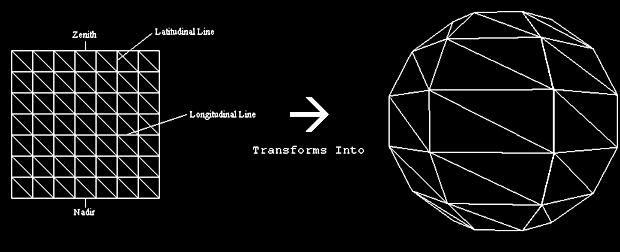
\includegraphics[width=\textwidth,height=\textheight,keepaspectratio]{resources/sphere05.jpg}
 	\captionsetup{type=figure, width=0.8\linewidth}
	\caption{Objetivo do algoritmo de construção de esfera}
\label{fig:ssec1:diagram:plane:to:sphere} 
\end{center}



\begin{center}
 	
 	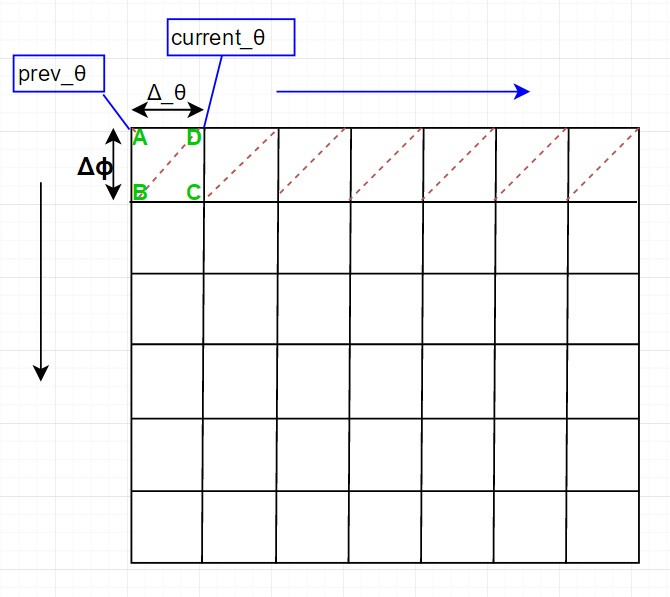
\includegraphics[keepaspectratio]{resources/esferaw.jpg}
 	\captionsetup{type=figure, width=0.8\linewidth}
	\caption{Diagrama de representativo de construção de esfera}
\label{fig:ssec1:diagram:sphere} 
\end{center}


No \emph{Figura~\ref{fig:ssec1:diagram:sphere}} pode-se ver uma matriz, que
representa a esfera nos graus de $\phi$ e $\theta$ para 6 \emph{stacks}
e 7 \emph{slices}. Assim como um mapa representativo da Terra, pretende-se
mostrar os pontos se a esfera fosse aplanada (ver
\emph{Figura~\ref{fig:ssec1:diagram:plane:to:sphere}}).

Em cada quadrícula são calculados 4 pontos iniciais, com base nos cálculos
apresentados pelo fórmula anterior. Note-se que, se usou duas variáveis para
guardar o $\phi$ anterior e o $\phi$ corrente, e $\theta$ anterior  e $\theta$
corrente. Adicionalmente é calculada a diferença de graus entre \emph{slices}
e \emph{stacks}, representados por $\Delta \phi$ e $\Delta \theta$,
respetivamente. 

A intenção é calcular cada quadricula para cada linha e coluna, com auxilio das
diferenças dos ângulos e à medida que se avança em cada quadricula, guardar
o último grau calculado ($\phi$ e $\theta$) e calcular nos pontos com
o incremento nestes ângulos. Assim desloca-se para a direita na matriz, conforme
$\theta$ avança de 0 para $2\pi$ e para baixo, conforme $\phi$ avança de
$\dfrac{\pi}{2}$ para $-\dfrac{\pi}{2}$ (sentido dos ponteiros do relógio).
O \emph{Algoritmo~\ref{alg:secc1:esfera}} representa este processo
e a \emph{Figura~\ref{fig:sec1:sphere:angles}} demonstra o que se
mencionou.  


\begin{center}
 	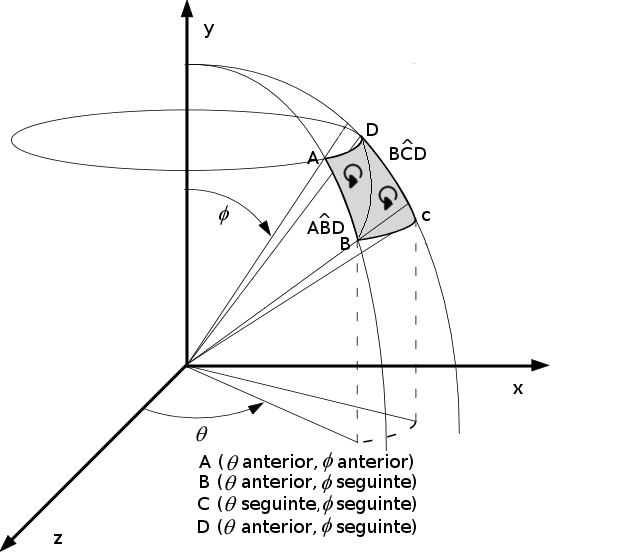
\includegraphics[width=\textwidth,height=0.5\textheight,keepaspectratio]{resources/esfera2.png}
 	\captionsetup{type=figure, width=0.8\linewidth}
	\caption{Diagrama de construção de esfera, com eixos, ordem do vértices
	e ângulos}
\label{fig:sec1:sphere:angles} 
\end{center}

O resultado pode-se ver na \emph{Figura~\ref{fig:ssec1:res:sphere}}, que
demonstra uma esfera em \emph{wireframe} gerada com a aplicação.  

\begin{center}
 	
 	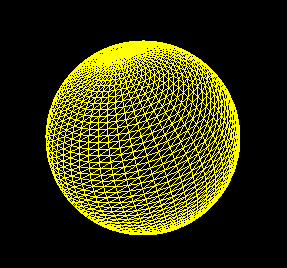
\includegraphics[keepaspectratio]{resources/sphere.png}
 	\captionsetup{type=figure, width=0.8\linewidth}
	\caption{Esfera gerada}
\label{fig:ssec1:res:sphere} 
\end{center}
\newpage

\newgeometry{margin=1cm}
\begin{landscape}
\thispagestyle{empty} %% Remove header and footer.

\begin{algorithm}
\caption{Esfera}\label{alg:secc1:esfera}

\begin{center}
%\footnotesize %% Smaller font size.

\begin{algorithmic}[1]
\State$\Delta\_\theta \gets \dfrac{2\pi}{slices}$

\State$\Delta\_\phi \gets \dfrac{2\pi}{stacks}$

\State$prev\_\phi \gets \dfrac{\pi}{2}$

\State$current\_\phi \gets prev\_\phi - \Delta\_\phi$


\State$i \gets 0$
\While{$i \leq stacks$} 


\State$prev\_\theta \gets 0$
\State$current\_\theta \gets \Delta\_\theta$

\State$j \gets 0$

\While{$j \leq slices$} 


\State$Ponto A \gets raio*\cos(prev\_\phi) * \sin(prev\_\theta)$, $
raio*\sin(prev\_\phi)$, $raio*\cos(prev\_\phi) * \cos(prev\_\theta)$
\State$Ponto B \gets raio*\cos(current\_\phi)*\sin(prev\_\theta)$,$
 raio*\sin(current\_\phi)$,$
 raio*\cos(current\_\phi) * \cos(prev\_\theta)$
\State$Ponto C \gets raio*\cos(prev\_\phi) * 
 \sin(current\_\theta),raio*\sin(prev\_\phi)$,$
 raio*\cos(prev\_\phi) * \cos(current\_\theta)$
\State$Ponto D \gets raio*\cos(current\_\phi) *
 \sin(current\_\theta)$,$raio*\sin(current\_\phi)$,$raio*\cos(current\_\phi) *  \cos(current\_\theta)$
\newline
\State$Triangulo(Ponto A, Ponto B, Ponto D)$ \Comment{Guardado em ficheiro}
\State$Triangulo(Ponto B, Ponto C, Ponto D)$ \Comment{Guardado em ficheiro}
\newline
\State$prev\_\theta \gets current\_\theta$
\State$current\_\theta \gets current\_\theta + \Delta\_\theta $
\newline
\State$j \gets j + 1$ 

\EndWhile{}

\State$prev\_\phi \gets Current\_\phi$
\State$current\_\phi \gets Current\_\phi - \Delta\_\phi $
\State$i \gets i + 1$ 

\EndWhile{}

\end{algorithmic}

\end{center}

\end{algorithm}

\end{landscape}
\restoregeometry{}


\newpage


\subsection{Disco}
Nesta secção descreve os procedimentos usados para desenvolver um disco.
A motivação para o desenvolvimento desta figura provém da necessidade de
representar os anéis que rodeiam os planetas Saturno e Úrano.


\subsubsection{Análise do Problema}

Existem certos elementos do sistema solar, que são característicos de um modelo
do mesmo: anéis e órbitas. Apesar do significado de ambos ser diferente, ambos
podem ser desenhados com o mesmo objeto, variando apenas no raio interno
e externo.

Com efeito, requer-se para este projeto que se criem discos de vários tamanhos
para os anéis de Saturno e Neptuno, e para as órbitas de cada planeta. Note-se
que cada anel tem que ter alguma espessura, uma vez que, num plano, no
\emph{OpenGL} não se consegue ver o objeto. Assim cada disco terá duas
circunferências, uma interior e outra exterior, com raio interno e externo
respetivamente. Assim, as duas circunferências têm os mesmos pontos \emph{xx}
e \emph{zz} mas com uma distancia fixa no eixo \emph{yy}. 

A fórmula para desenhar uma circunferência está representada na
\emph{Equação~\ref{eq:equ3}} 

\begin{equation}
\begin{cases}
			x =  \sin(\theta) * r \\
	    z =  \cos(\theta) * r
\end{cases}
\label{eq:equ3}
\end{equation}



Nesta secção apresentam-se diagramas que explicam o processo de criação de uma
disco.

A \emph{Figura~\ref{fig:ssec1:disc}} representa a forma como a iteração será
feita, bem como apresenta de lado a espessura do disco.


\begin{center}
 	
 	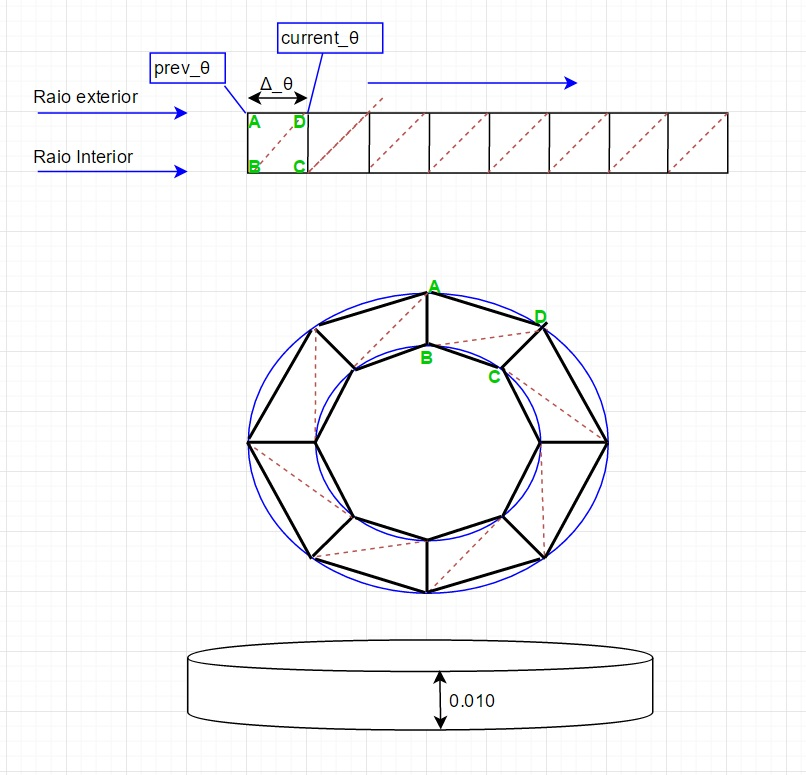
\includegraphics[width=\textwidth,height=\textheight,keepaspectratio]{resources/disco.jpg}
 	\captionsetup{type=figure, width=0.8\linewidth}
	\caption{Diagrama Disco}
\label{fig:ssec1:disc} 
\end{center}

Como se pode verificar o diagrama é relativamente semelhante ao da esfera.
A matriz aqui observada apenas tem uma linha porque não se consideram
\textit{stacks} na representação do disco. As 8 colunas que representam as
8 \textit{slices} (estas 8 slides servem meramente para propósitos
exemplificativos). 


\begin{center}
 	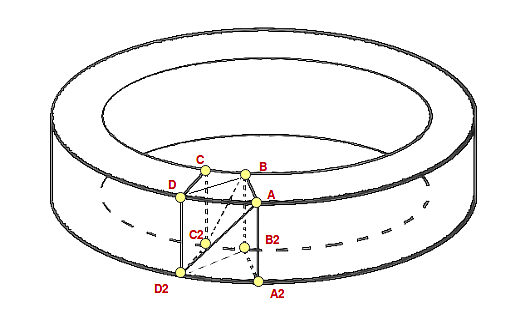
\includegraphics[width=\textwidth,height=0.5\textheight,keepaspectratio]{resources/discodiagram.png}
 	\captionsetup{type=figure, width=0.8\linewidth}
	\caption{Pormenor dos vértices para desenho de um disco}
\label{fig:sec1:disc:vertex} 
\end{center}

Como se pode observar, o raciocínio é desenhar quadricula a quadricula com dois
triângulos cada, neste exemplo verifica-se que a primeira quadricula
é constituída pelos triângulos ABD e BCD.\ As coordenadas de cada ponto (vértice
dos triângulos) são calculados com o auxílio das variáveis angulares
prev\_$\theta $ e current\_$\theta$ usando a formulação das coordenadas
esféricas. A diferença entre esta é o comprimento/largura da quadricula que
corresponde a $\dfrac{2\pi}{slices}$. 

Ora este processo é referente à face superior do disco. Para desenhar a face
inferior faz-se o mesmo processo mas com outros vértices equivalentes nos eixos
\emph{xx} e \emph{zz} mas com uma diferença fixa de 0.010 \emph{yy} para
representar a altura.

Quanto à face lateral do disco o processo é idêntico ao representado na matriz
acima, mas enquanto que, para representar tanto a face superior como a inferior,
os pontos usados têm todos os o mesmo valor \emph{yy}, para representar o lado do disco
usa-se uma combinação dos pontos de ambas as faces. 

Este processo está representado no \emph{Algoritmo~\ref{alg:sec1:disco}},
e um resultado figura na \emph{Figura~\ref{fig:sec1:disc:res1}} e na
\emph{Figura~\ref{fig:sec1:disc:res2}}.  

\begin{center}
 	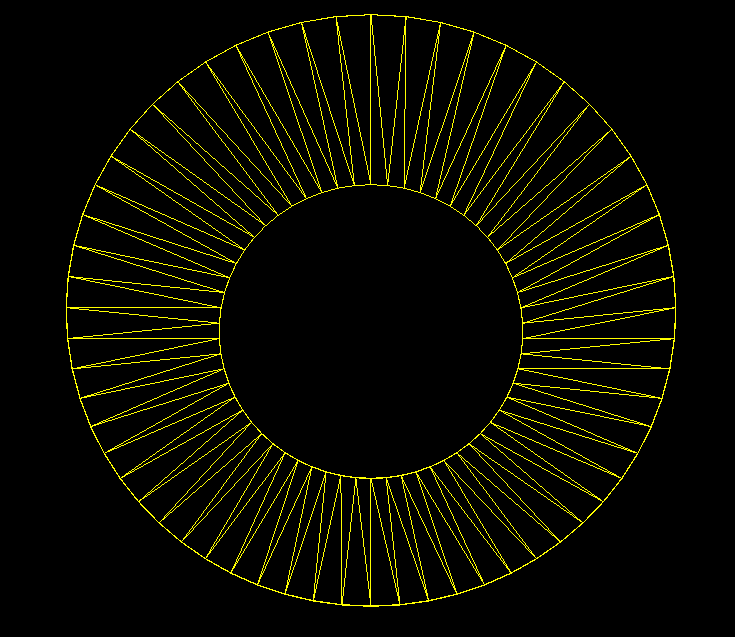
\includegraphics[width=\textwidth,height=0.5\textheight,keepaspectratio]{resources/disco1.png}
 	\captionsetup{type=figure, width=0.8\linewidth}
	\caption{Resultado de um disco em \emph{wireframe}, visto de baixo}
\label{fig:sec1:disc:res1} 
\end{center}


\begin{center}
 	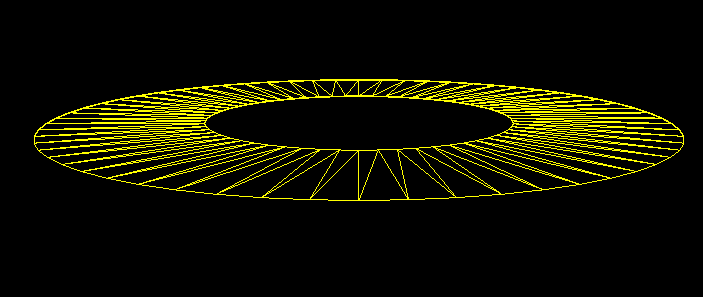
\includegraphics[width=\textwidth,height=0.5\textheight,keepaspectratio]{resources/disco2.png}
 	\captionsetup{type=figure, width=0.8\linewidth}
	\caption{Resultado de um disco em \emph{wireframe}, visto de outro ângulo}
\label{fig:sec1:disc:res2} 
\end{center}




\newgeometry{margin=1cm}
\begin{landscape}
\thispagestyle{empty} %% Remove header and footer.
\begin{algorithm}
\caption{Disco}\label{alg:sec1:disco}

\begin{center}
%\footnotesize %% Smaller font size.

\begin{algorithmic}[1]
\State$\Delta\_\theta \gets \dfrac{2\pi}{slices}$


\State$prev\_\theta \gets 0$
\State$current\_\theta \gets \Delta\_\theta$

\State$i \gets 0$


\While{$i \leq slices$} 

\State$Ponto A \gets raioOut*\sin(prev\_\theta),
 0.005,
 raioOut*\cos(prev\_\theta)$

\State$Ponto B \gets raioIn*\sin(prev\_\theta),
 0.005,
 raioIn*\cos(prev\_\theta)$

\State$Ponto C \gets raioIn*\sin(current\_\theta),
 0.005,
 raioIn*\cos(current\_\theta)$

\State$Ponto D \gets raioOut*\sin(current\_\theta),
  0.005,
 raioOut*\cos(current\_\theta)$

\State$Ponto A2 \gets raioOut*\sin(prev\_\theta),
 -0.005,
 raioOut*\cos(prev\_\theta)$

\State$Ponto B2 \gets raioIn*\sin(prev\_\theta),
 -0.005,
 raioIn*\cos(prev\_\theta)$

\State$Ponto C2 \gets raioIn*\sin(current\_\theta),
 -0.005,
 raioIn*\cos(current\_\theta)$

\State$Ponto D2 \gets raioOut*\sin(current\_\theta),
  -0.005,
 raioOut*\cos(current\_\theta)$




\Comment{Lado de cima}

\State$Triangulo(Ponto D, Ponto B, Ponto A)$ \Comment{Guardado em ficheiro}
\State$Triangulo(Ponto C, Ponto B, Ponto D)$ \Comment{Guardado em ficheiro}



\Comment{Lado de baixo}
\State$Triangulo(Ponto A2, Ponto B2, Ponto D2)$ \Comment{Guardado em ficheiro}
\State$Triangulo(Ponto D2, Ponto B2, Ponto C2)$   \Comment{Guardado em ficheiro}
		  
\Comment{Lado de externo}
\State$Triangulo(Ponto A2, Ponto A, Ponto D2)$\Comment{Guardado em
ficheiro}
\State$Triangulo(Ponto D, Ponto D2, Ponto A)$\Comment{Guardado em
ficheiro}
  
\Comment{Lado de interno}
\State$Triangulo(Ponto B, Ponto C2, Ponto B2)$\Comment{Guardado em
ficheiro}
\State$Triangulo(Ponto C, Ponto C2, Ponto B)$\Comment{Guardado em
ficheiro}



\State$prev\_\theta \gets current\_\theta$
\State$current\_\theta \gets current\_\theta + \Delta\_\theta$

\State$i \gets i + 1$


\EndWhile{}
\end{algorithmic}
\end{center}

\end{algorithm}


\end{landscape}
\restoregeometry{}

\clearpage

\section{Motor}

Nesta secção pretende-se descrever o funcionamento do Motor \emph{Engine},
e para tal pretende-se abordar vários aspetos desde as estruturas de dados
auxiliares, estruturas de dados para os diferentes tipos de objetos que compõem
o motor, descrição do processo de leitura e do processo de \emph{rendering}.
Para este projeto usaram-se \emph{vertex array objets} para o \emph{rendering}
das geometrias, tanto vértices, vetores normais, como também coordenadas de
textura.


\subsection{Estruturas de dados auxiliares}


Para poder manipular dos dados, tanto dos vértices, normais, coordenadas de
textura, como também informação sobre os \emph{vertex array objets --- VBOs},
luzes com as suas propriedades, identificadores de texturas e ainda a raiz da
estrutura de dados para armazenar informação do ficheiro XML, criou-se um tipo
de dados \emph{Models}. 

Este tipo de dados é composto por vários \texttt{vector}, dos quais um para os
vértices, outro para os vetores normais e outro para coordenadas de textura.
Note-se que estes vetores contêm os identificadores para a inicialização
e \emph{rendering} dos VBO's, sendo que a informação para o \emph{rendering} dos
VBO's se encontra num tipo de dados homónimo, com um índice para os
\texttt{vector} para e o total de vértices. De salientar que o valor de índice
e do número de vértices é partilhado pelos diferentes VBO's, de vértices,
normais e texturas, uma vez que o número de ocorrência de vértices, normais
e pontos da textura são os mesmos, e consequentemente, o acesso por índice
a cada um dos \emph{vector} de identificadores é igual. Porém, na função de
inicialização, no preenchimento do \emph{buffer} com os valores para cada tipo
de objeto foi multiplicado o número de componentes (coordenadas) de cada
vértices. Assim para normais e vértices o número de vértices foi multiplicado
por três, e para as coordenadas das textura, o número de vértices foi
multiplicado por 2.

Para cada ficheiro com informação sobre a geometria, existe um e um só
\texttt{VBO} (o tipo de dados), uma vez que a mesma geometria pode ser usadas
várias vezes. Assim existe uma tabela com o nome do ficheiro como chave, tendo
associado o tipo \texttt{VBO} a essa chave. Para as texturas, a estrutura
é similar, só que para cada nome do ficheiro da imagem está associado um número
inteiro não negativo para o identificador da textura. 

Relativamente, à informação de luzes e suas componentes existe um vetor do tipo
\texttt{Light*}, cujo o tipo contém informação sobre as luzes, e posteriormente
neste documento será melhor documentado. Ainda para as luzes, dado que o OpenGL,
na definição de propriedades materiais de cada geometria, essa propriedade
é partilhada de forma global até ser novamente alterada, criou-se um vetor do
tipo \texttt{Materials*} para armazenamento dos valores por defeito da
propriedades de materiais. Assim, após a definição de uma propriedade de uma
material de uma geometria, este vetor é percorrido aplicando as propriedades
materiais por defeito.

Por último, ainda existe uma variável do tipo inteiro par controlo da atribuição
do índice do identificador do VBO's, e raiz para a estrutura de dados com
a informação me memória do ficheiro XML.\ 


\subsection{Estruturas de dados --- classes}

As classes definidas neste projeto servem o propósito de abstrair os conceitos
de computação gráfica como transformações geométricas, definição de luzes e suas
propriedades, bem como classes auxiliares para representação de tipos
geométricos como pontos em 3 dimensões e 4 dimensões e valores RGBA (\emph{red,
green, blue, alpha}).


Para definir a componente de luz material de cada geometria, para além das
normais é necessário definir as quatro características materiais de reflexão da
luz na geometria, tanto componente físicas reais (componente difusa
e especular), como virtuais (ambiente e emissiva). As componentes ambiente
e emissiva são virtuais, uma vez que, não é possível representar a luz ambiente
de uma cena, nem se um objeto emite luz (componente emissiva) e, como tal, não
dependem dos valores dos vetores normais à superfície da geometria.

Para todas as características dos materiais foram definidas classes, numa
hierarquia, e à exceção da componente especular, apenas aplicam um conjunto de
valores representativo dos valores RGBA.\ No entanto, o contexto da sua aplicação
é diferente, uma vez que é invocado a função \texttt{glMaterialfv} com
a respetiva componente (\texttt{GL\_EMISSIVE}, \texttt{GL\_DIFFUSE},
\texttt{GL\_AMBIENT} e \texttt{GL\_SPECULAR}) e é aplicado aquando da invocação
do método \texttt{applyProperties} ou a partir da superclasse \emph{Materials}
ou partir de uma instância da própria classe. A componente especular possui
ainda o brilho da componente especular (\emph{shininess}).A Figura~\ref{ig:ssec2:mat}
apresenta parte da hierarquia de classes mencionada.


\begin{center} 	
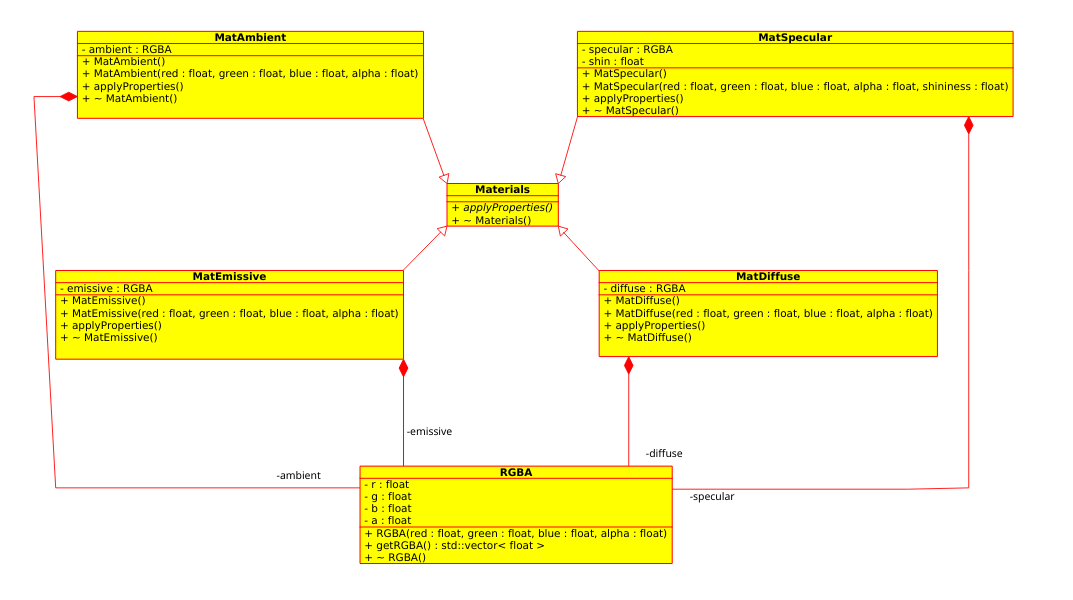
\includegraphics[width=\textwidth,height=\textheight,keepaspectratio]{resources/material.png}
\captionsetup{type=figure, width=0.8\linewidth}
\caption{Hierarquia de classes de \emph{Materials}} 
\label{fig:ssec2:mat} 
\end{center}

Para definir as luzes, podem ser definidas até um conjunto de 8 luzes (assumindo
uma abordagem de luzes fixas ao espaço global), podendo estas luzes posicionais 
(\texttt{FixedLight}), direcionais (\texttt{DirectionalLight}) ou
\emph{spotlight} \texttt{Spolight}. Cada um desde tipos de luz pode ter várias
componentes, tais como as geometrias, neste caso apenas sendo três: difusa,
ambiente e especular.

Tal como para as caraterísticas materiais, cada classe possui um conjunto de
valores RGBA, sendo cada característica da luz aplicada no seu contexto com
a função \texttt{glLight}, com o identificador da luz a que estão associadas,
com a componente correspondente (\texttt{GL\_DIFFUSE}, \texttt{GL\_AMBIENT}
e \texttt{GL\_SPECULAR}) através da superclasse \texttt{LightProperty} ou duma
instância da própria classe, à semelhança da hierarquia anterior. Note-se que,
aqui não faz sentido colocar o brilho da reflexão.


\begin{center} 	
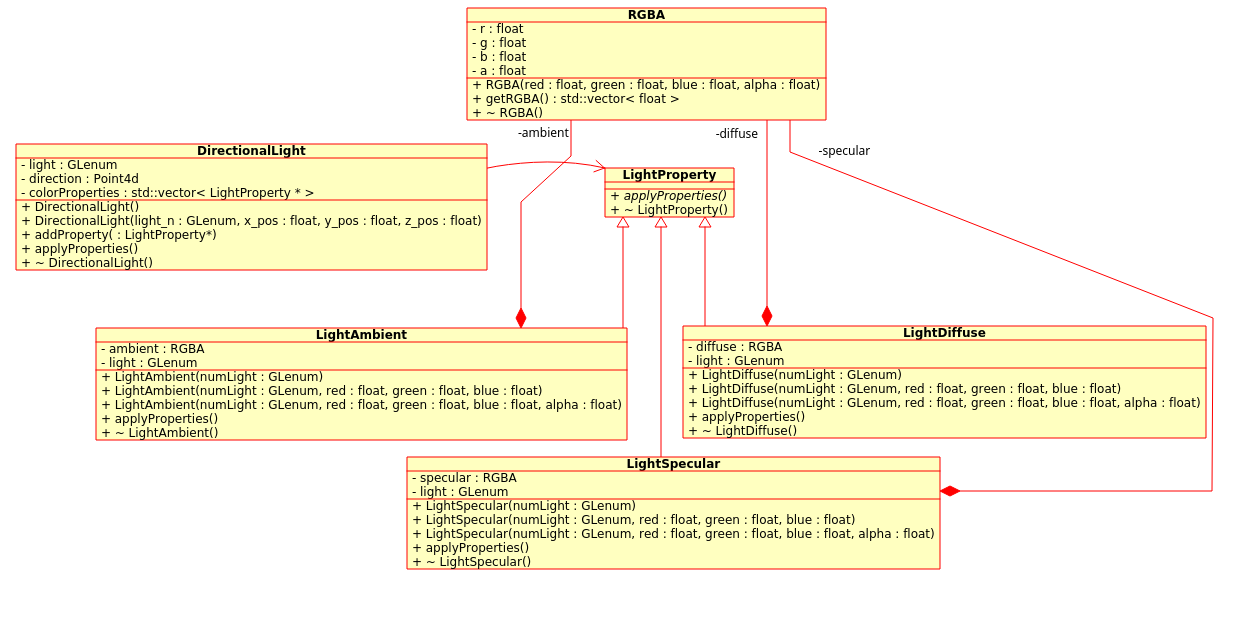
\includegraphics[width=\textwidth,height=\textheight,keepaspectratio]{resources/lightProperties.png}
\captionsetup{type=figure, width=0.8\linewidth}
\caption{Hierarquia de classes de \emph{LightProperty}} 
\label{fig:ssec2:props} 
\end{center}

Relativamente ao tipo de luzes, estes podem ser de três tipos: direcional,
posicional e \emph{spotlight}. Cada um deste tipos possui um número variado de
parâmetros, que caraterizam cada tipo de luz. 

A luz direcional apenas é parametrizada pelo identificador da luz e pela direção
da luz, sendo 3 coordenadas do referencial ortonormado, mais a coordenada $w$
(coordenadas homogéneas), com o valor 0, o que representa um vetor. Uma vez que
uma luz direcional pode ser considerada com uma luz infinitamente longe, esta
não possui parâmetros de atenuação, no entanto, possui as propriedades da luz
mencionadas atrás.

Relativamente à luz posicional, à semelhança da luz direcional, para além do
identificador da luz, recebe as coordenadas homogêneas, no entanto a coordenada
$w$ tem um valor de 1, dado que é um ponto. Nesta luz já se podem definir
valores de atenuação, sendo estes valor da atenuação constante, linear ou
quadrática. O inverso da soma deste valores, sendo o valor de atenuação
quadrática multiplicado pelo quadrado da distância entre o ponto de luz
e o vértice de uma geometria e valor da atenuação linear multiplicado pela
distância, é o fator de atenuação. Esta relação está
representada na Equação~\ref{eq:atenuation}.

\begin{equation}
	fator de atenuação = \frac{1}{k_c + k_{l}d + k_{q}d^2}
\label{eq:atenuation}
\end{equation}

Na Equação~\ref{eq:atenuation} $k_c$ é a atenuação constante, $k_l$
é a atenuação linear, $k_q$ é a atenuação quadrática e $d$ é a distância entre
a posição da luz e o vértice da geometria. No OpenGL a característica da
atenuação, pode ser definida pela função \texttt{glLightf}, com o identificador
da luz, podendo ser \texttt{GL\_CONSTANT\_ATENUATION},
\texttt{GL\_LINEAR\_ATENUATION} e \texttt{GL\_QUADRATIC\_ATENUATION}, para
atenuação constante, linear e quadrática respetivamente.

Por último, temos a luz do tipo \emph{spotlight}. Este tipo de luz, para além do
identificador da luz e da posição da mesma, possui uma direção para onde o cone
de luz está apontado e o ângulo de abertura do cone, estando este último a 180º
por defeito, podendo ser alterado para um valor entre 0 e 45º. Adicionalmente,
existe um expoente de concentração de luz. Do mesmo modo, que as anteriores
luzes, possui contribuições do tipo especular, ambiente e difuso.


As coordenadas homogéneas são representadas pela classe \texttt{Point4d}.
À semelhança as outras hierarquias de classes já descritas, existe uma
superclasse (\texttt{Light}) sendo as características de cada tipo de luz,
aplicadas pela função \texttt{applyProperties} no contexto desta superclasse, ou
numa instância de cada uma das subclasses. Cada uma das classes implementa
a função \texttt{glLightsfv}, aplica as contribuições e ativa a luz, no método
\texttt{applyProperties}, nesta ordem. Adicionalmente, existe uma método
\texttt{addProperty}, que adiciona as contribuições de natureza especular,
difusa ou ambiente. A hierarquia de classes pode ser vista em maior detalhe na
Figura~\ref{fig:ssec2:lights}.


\begin{center} 	
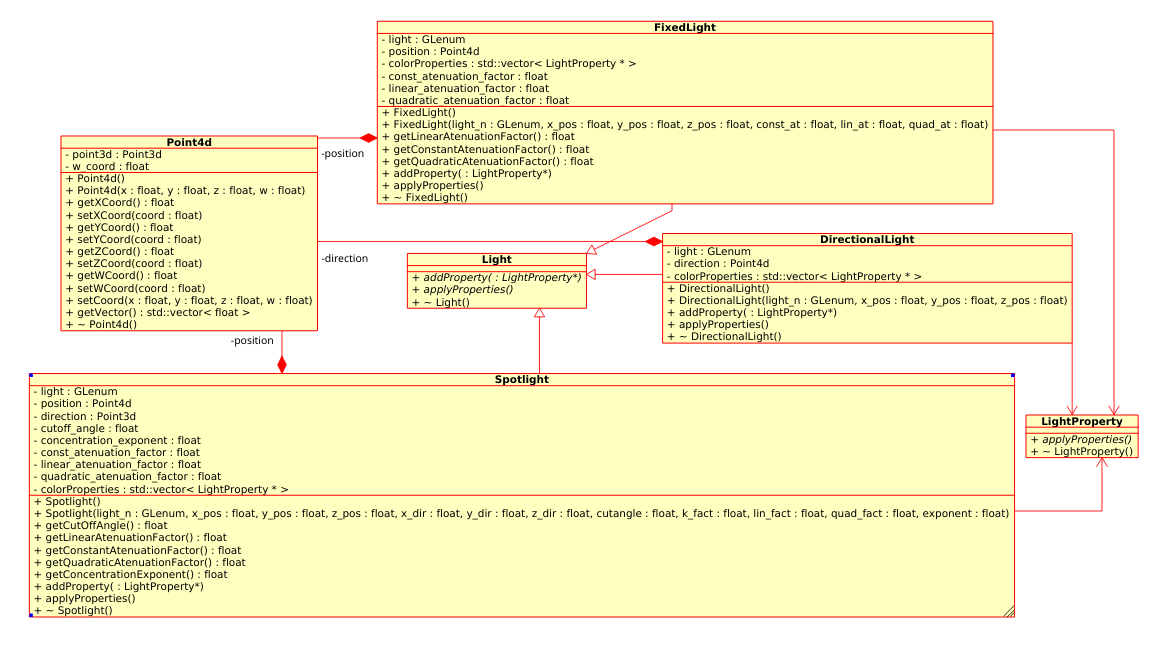
\includegraphics[width=\textwidth,height=\textheight,keepaspectratio]{resources/light.png}
\captionsetup{type=figure, width=0.8\linewidth}
\caption{Hierarquia de classes de \emph{Light}} 
\label{fig:ssec2:lights} 
\end{center}


\subsection{\emph{Vertex Array Objects}}

O OpenGL possibilita dois modos de renderização: o modo imediato
e o \emph{vertex buffer objects} (VBOs). Os VBOs permitem um ganho substancial
de performance, uma vez que os dados são logo enviados para a memória da placa
gráfica onde residem, e por isso podem ser renderizados diretamente da placa
gráfica. O modo imediato usa a memória do sistema onde os dados são inseridos
\emph{frame} a \emph{frame}, usando uma API de renderização, o que causa peso
computacional sobre o processador.


Para a utilização das VBO's é necessário recorrer a criação de \emph{arrays} com
os dados para renderizar geometria, com vetores normais para as luzes
e coordenadas de textura, para uma eventual aplicação desta. Com efeito,
é necessário, em primeiro lugar, ativar os \emph{arrays} com os diferentes tipos
de dados e colocar os dados num \emph{buffer object}. Estes \emph{arrays} são
acedidos pelo seu endereço individual da sua localização em memória, sendo então
desenhadas as figuras geométricas dos respetivos conteúdos dos \emph{arrays}.


Note-se que, no OpenGl, qualquer inteiro sem sinal pode ser usado como um
identificador de \emph{buffer objecto}. Estes identificadores podem-se
armazenados numa estrutura, sendo necessário, em seguida, gerar \emph{buffers}
para os vértices, para os vetores normais e coordenadas de textura (um
\emph{buffer} para cada \emph{array} --- vértices, normais e coordenadas de
textura) \texttt{glGenBuffers} e ativar cada \emph{buffer} pelo seu
identificador (\texttt{glBindBuffer}) e preencher o \emph{buffer} com os dados
de cada \emph{array} previamente mencionado.


Para desenhar, a figura geométrica é necessário definir a semântica, ou seja,
definir o \emph{offset} relativo ao inicio do buffer consoante o tipo de dados,
fazer o bind do objeto apropriado para fazer a renderização dos \emph{arrays} de
vértices, normais e coordenadas de textura usando a função adequada
(\texttt{glDrawArrays} ou \texttt{glDrawElements}).De notar que, cada
\emph{bind} é seguido da semântica. A semântica para os vértices é feita usando
a função \texttt{glVertexPointer}, definido o valor 3 o número de elementos do
tipo valor de vírgula flutuante, correspondente às coordenadas de cada vértice.
Relativamente à semântica para os vetores normais, é utilizada a função
\texttt{glNormalPointer}. Nesta função não é necessário definir o número de
coordenadas, uma vez que a própria função já o faz. No entanto, é necessário
definir o tipo, como valor de vírgula flutuante. Por último, para as coordenadas
das texturas é necessário definir a semântica com a função
\texttt{glTexCoordPointer}, onde o número de elementos para cada vértice será
dois, dado que as textura são bidimensionais. Note-se também, que é necessário
fazer o \emph{bind} da textura pelo identificador obtido pela
função \texttt{loadTexture} antes de proceder ao \emph{rendering} da geometria,
sendo invocada logo de seguida o \emph{bind} para identificador 0, para evitar
que continua a desenhar a mesma textura. Este processo é feito na função
\texttt{drawElement}, que será descrito mais à frente. A inicialização dos
\emph{buffers} é feita pela função \texttt{initBuffers} e para o processo de
\emph{rendering} utilizou-se a função \texttt{drawVBO}, que faz o \emph{bind}
e define a semântica, que é aplicada na função \texttt{drawElement} que aplica
outros elementos para o desenho da geometria, como o \emph{bind} da textura
mencionado acima e aplicação de cores dos materiais, \emph{reset} do mesmos.  


\subsection{Descrição do processo de leitura}


A função de leitura identifica \emph{tags} correspondentes às transformações
geométricas, sejam elas animadas ou estáticas, e à medida que se vai lendo
o ficheiro XML, vai se construindo uma árvore n-ária do tipo \texttt{Group},
como demonstra a Figura~\ref{fig:ssec2:strut}. No entanto, existem dois tipos de
elementos do XML com interesse particular neste projeto, que são os
\texttt{models} e as \texttt{lights}.  

\begin{center} 	
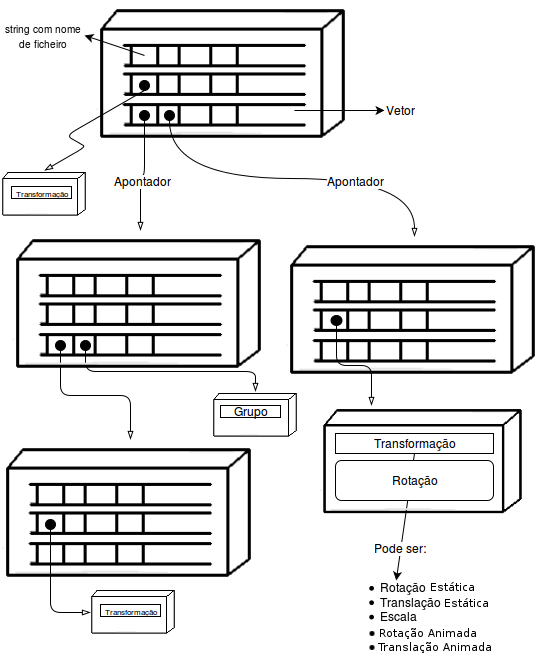
\includegraphics[width=\textwidth,height=\textheight,keepaspectratio]{resources/estrutura.png}
\captionsetup{type=figure, width=0.8\linewidth}
\caption{Árvore \emph{n-ária} para armazenamento de grupos}
\label{fig:ssec2:strut} 
\end{center}

\subsubsection{Modelos}

Para o caso de ocorrência da \emph{tag} \texttt{models}, para cada ocorrência de
uma \emph{tag} filha \texttt{model}, a função \texttt{readXMLFromRootElement}
obtém o nome do ficheiro de vértices, normais e coordenadas de textura. Se
a \emph{tag} \texttt{model} também tiver um atributo \texttt{texture}, para cada
propriedade material, cria a propriedade material de acordo com a ocorrência
(\texttt{diffuse}, \texttt{ambient}, \texttt{specular} e \texttt{emissive}).
Note-se que, se alterou o ficheiro XML para conter \emph{tags} desta forma,
dado que:  é mais legível; mais fácil de tratar cada caso na leitura. Em
seguida, é guardado o nome do ficheiro 3d no vetor de nomes de modelos no tipo
\texttt{Group}, bem como o conjunto de propriedades materiais e nome do ficheio
de textura. Note-se que, pode não existir uma ocorrência de uma textura, ou de
propriedades materiais. No entanto, por uma questão de manter a representação
ordenada para ser acedida por índice, caso não haja uma ocorrência de um
ficheiro de textura, é adicionada a \emph{string} vazia ou o vetor vazio.

Caso o nome da textura existir, isto é, não for uma \emph{string} vazia,
é carregada a textura com a função \texttt{loadTexture}, que devolve um
identificador depois de fazer o \emph{bind} da textura, que ocorre na função
\texttt{loadTexture}. O nome do ficheiro da textura e identificador são
guardados num par chave/valor na estrutura \texttt{Models} mencionada no início
do capítulo. Em seguida é invocada a função \texttt{readFile}, que procederá
a leitura do ficheiro 3d, inserirá um par chave/valor na tabela para o efeito em
\texttt{Models}, com o nome do ficheiro 3d e o tipo \texttt{VBO}, que por sua
vez possui o índice dos vetores de identificadores de \emph{buffers} (vértices,
normais e coordenadas de textura) --- um índice para os três vetores, como já
foi explicado ---, e inicializará os \emph{vertex array objects}.      



\subsubsection{Luzes}

Relativamente às luzes, neste modelo são descritas fora de um grupo, no entanto,
a função de leitura permite a flexibilidade de ter luzes dentro de um grupo.
Mesmo assim, pretende-se que as luzes sejam declaradas no inicio do ficheiro do
documento XML, uma vez que os atributos das luzes e seus tipos são armazenados
numa estrutura à parte (\texttt{Models}), para serem invocadas na
\texttt{renderScene} após o \texttt{gluLookAt}, antes de quaisquer
transformações geométricas, de forma as luzes ficarem fixas no espaço global.

Com efeito, para cada ocorrência da \emph{tag} \texttt{lights}, para cada
elemento \texttt{light} filho, se o tipo (\texttt{type}) for do valor
\texttt{DIR}, cria uma luz direcional, se for do valor \texttt{POINT} cria uma
luz posicional e se for do tipo \texttt{SPOT}, cria um \emph{spotlight}. Para
cada uma desta ocorrências, se existirem propriedades da luz, à semelhança da
propriedades materiais, cada componente é criado conforme a ocorrência
(\texttt{diffuse}, \texttt{specular} e \texttt{ambient}). Estas
componentes são adicionadas à luz, no entanto, podem não existir componentes da
luz, e nesse caso nada é adicionado. A luz é adicionada ao vetor de
\texttt{Light*} em \texttt{Models}.  



\subsection{Descrição do ciclo de \emph{rendering}}



Para fazer o \emph{rendering} da estrutura de dados em memória, implementou-se
uma função de travessia da árvore, colocada na função \texttt{renderScene}, após
a função \texttt{glLoadIndentity} e \texttt{gluLookAt}, nesta sequência.

Com efeito, a primeira instrução é a \texttt{glPushMatrix}, uma vez que se
pretende colocar uma matriz para aplicação das transformações no topo da
\emph{stack} de matrizes do \emph{OpenGL}. Em seguida, para cada transformação
contida num \texttt{Group}, é invocada a função \texttt{applyTrasformation}, que
aplica as transformações as transformações geométricas.

Em seguida, é invocada a função \texttt{drawElement}. Esta função especifica a primitiva
para que será criada com os vértices, normais e coordenadas de textura em
memória, usando a função \texttt{drawVBO}. Adicionalmente, itera pelas as
estruturas de \texttt{Group} (vetores de nomes de ficheiros 3d, vetor de vetor
de \texttt{Materials*}) e procura pela chave do nome do ficheiro, 3d ou textura,
o valor do tipo \texttt{VBO} e identificador da textura, respetivamente, nas
tabelas em \texttt{Models}. Caso o nome do ficheiro 3d existir é que invoca,
a função \texttt{drawVBO}, e antes disso, verifica se o nome da textura existe,
e só se existir é que faz o \emph{bind} da textura. A primeira estrutura a ser
iterada é o vetor de vetores de \emph{Materials*}, sendo que para cada valor de
vetor de \emph{Materials*}, as propriedades são aplicadas conforme o contexto,
pela a invocação do método da superclasse \texttt{applyProperties}. Após
o \emph{rendering} dos \emph{vertex array objects}, todas as propriedades
materiais por defeito do OpenGL são aplicadas, para evitar que propriedades de
diferentes geometrias, sejam aplicadas de forma transversal, até que sejam
alteradas novamente, que a aplicação dos valores por defeito faz.   

Como já foi mencionado, a aplicação das luzes acontece na \texttt{renderScene},
após o \texttt{gluLookAt} e antes da função \texttt{traverseTree} que possui
a descrição do modelo XML em memória. Para a aplicação das luzes aplica-se
o mesmo principio de utilização da hierarquia de classes que se usou até aqui,
e para cada ocorrência de uma instância de \texttt{Light*} no vetor em
\texttt{Models} é invocada a função \texttt{applyProperties} de \texttt{Light},
sendo a mesma função aplicada, no seu devido contexto nas subclasses.



\clearpage

\section{Resultados}



Os resultados obtidos estão nas imagens seguintes.

\begin{center}
 	
 	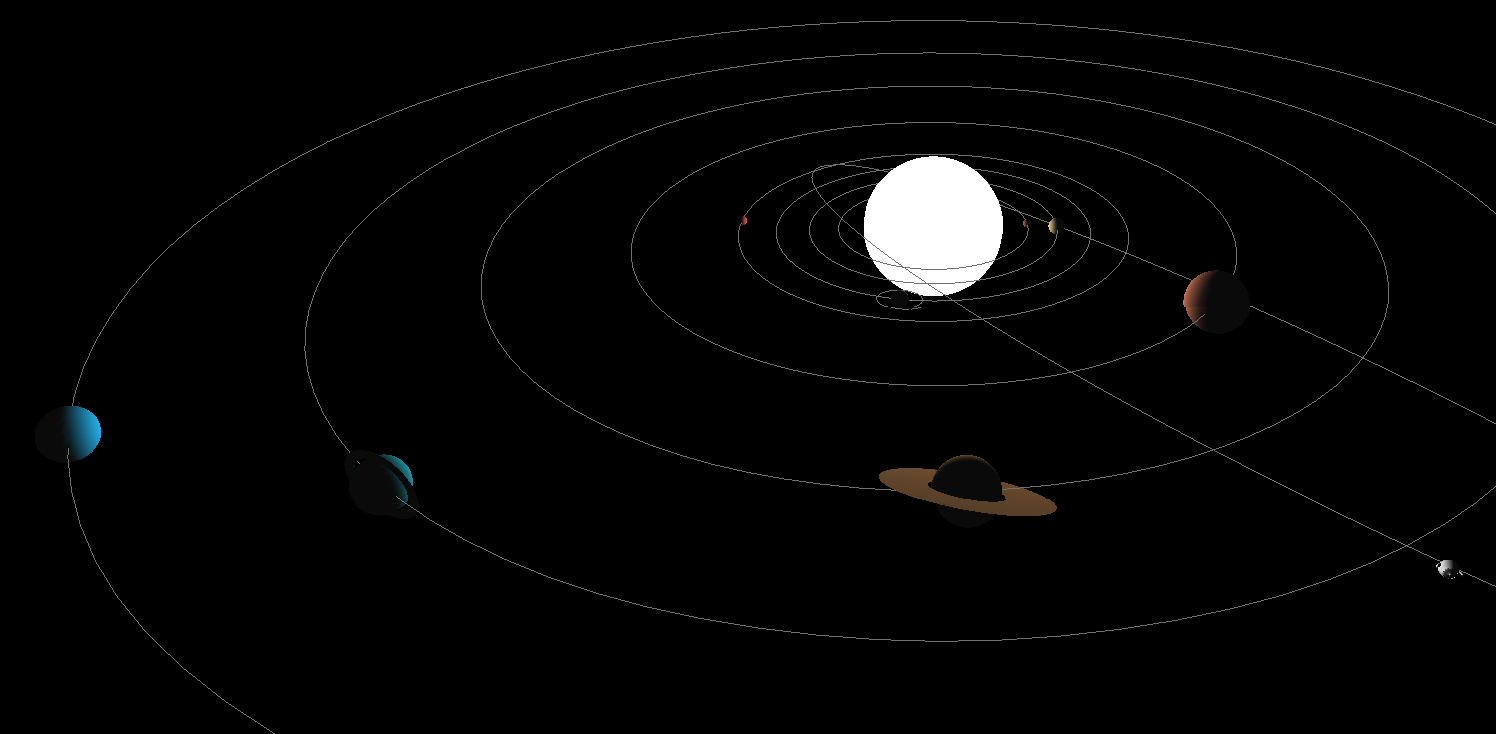
\includegraphics[width=\textwidth,height=\textheight,keepaspectratio]{resources/sistemaRGBA.png}
 	\captionsetup{type=figure, width=0.8\linewidth}
	\caption{\textit{Rendering} do modelo com cores e um luz posicional}
\label{fig:ssec3:tilt} 
\end{center}


\begin{center}
 	
 	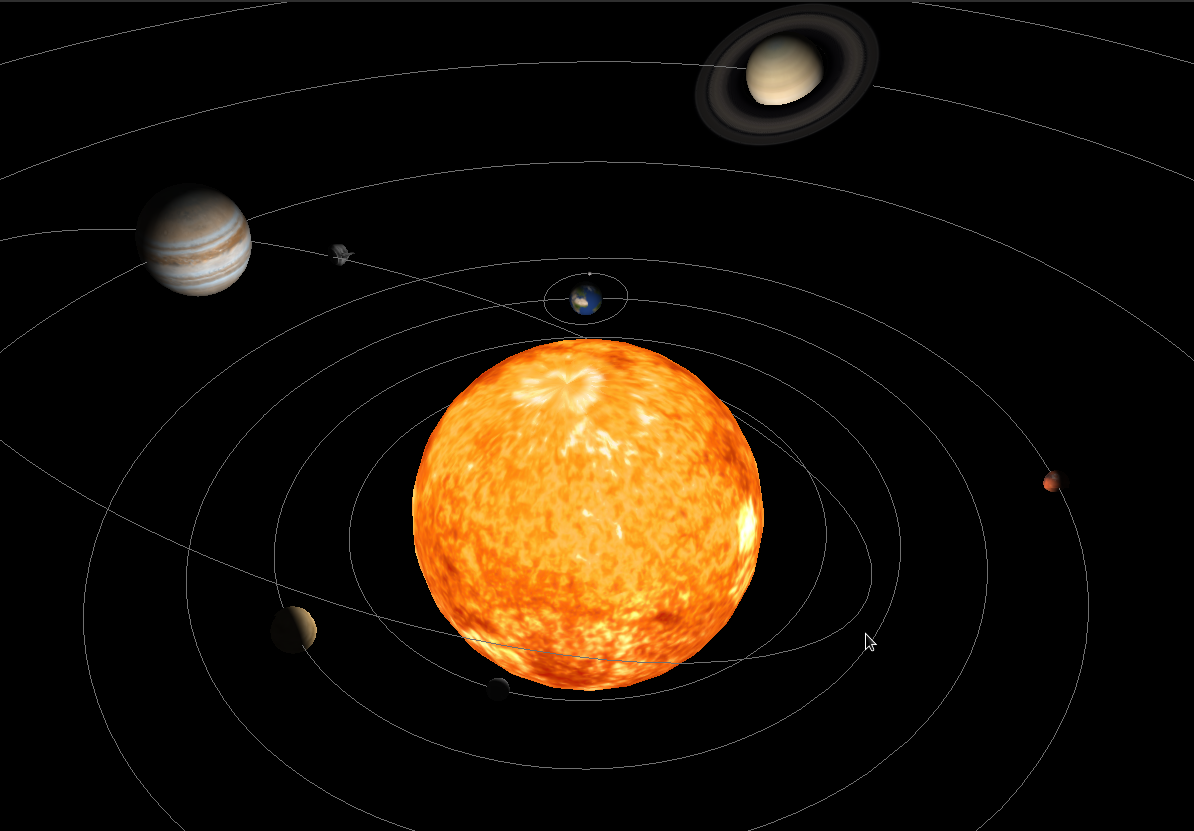
\includegraphics[width=\textwidth,height=\textheight,keepaspectratio]{resources/sistemaSolar.png}
 	\captionsetup{type=figure, width=0.8\linewidth}
	\caption{\textit{Rendering} do modelo com texturas e um luz posicional}
\label{fig:ssec3:tilt} 
\end{center}


A \emph{Figura~\ref{fig:ssec3:modelo}} mostra o modelo com cometa. 

\begin{center}
 	
 	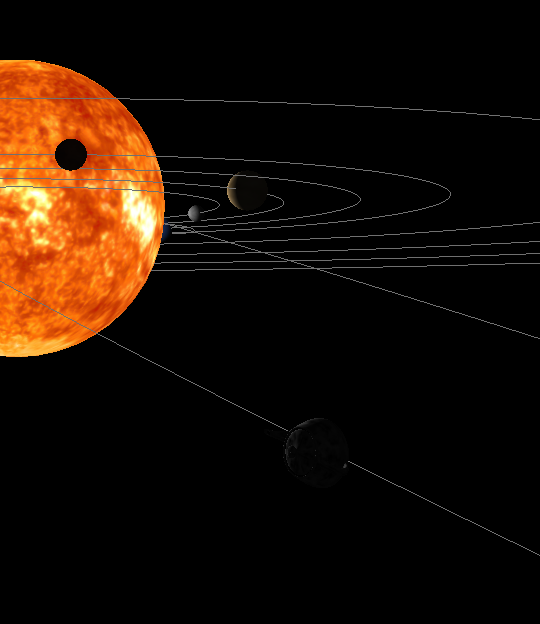
\includegraphics[width=\textwidth,height=\textheight,keepaspectratio]{resources/pormenorCometa.png}
 	\captionsetup{type=figure, width=0.8\linewidth}
	\caption{\textit{Rendering} do modelo com foco no cometa}
\label{fig:ssec3:modelo} 
\end{center}


\begin{center}
 	
 	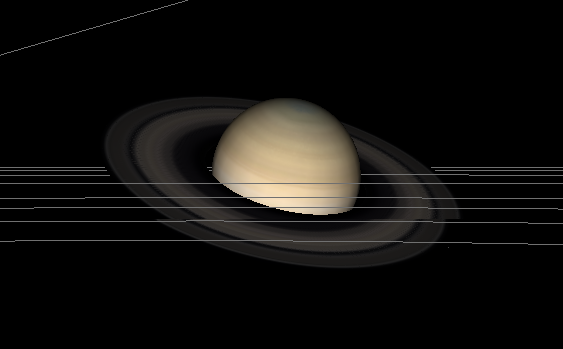
\includegraphics[width=\textwidth,height=\textheight,keepaspectratio]{resources/pormenorSaturno.png}
 	\captionsetup{type=figure, width=0.8\linewidth}
	\caption{\textit{Rendering} do modelo com foco em Saturno}
\label{fig:ssec3:modelo2} 
\end{center}




\clearpage

\section{Bezier}

Uma curva bezier pode ser definida por um qualquer numero de pontos, pontos estes chamados pontos de controlo da curva. Transformações como translação e rotação podem ser aplicadas na curva manipulando estes pontos. 

O algortimo de Casteljau oferece uma construção geométrica de onde se pode dividir uma curva de Bezier em duas curvas Bezier num parâmetro arbitrário t [0,1]. Como se pode observar:

\begin{center}
 	
 	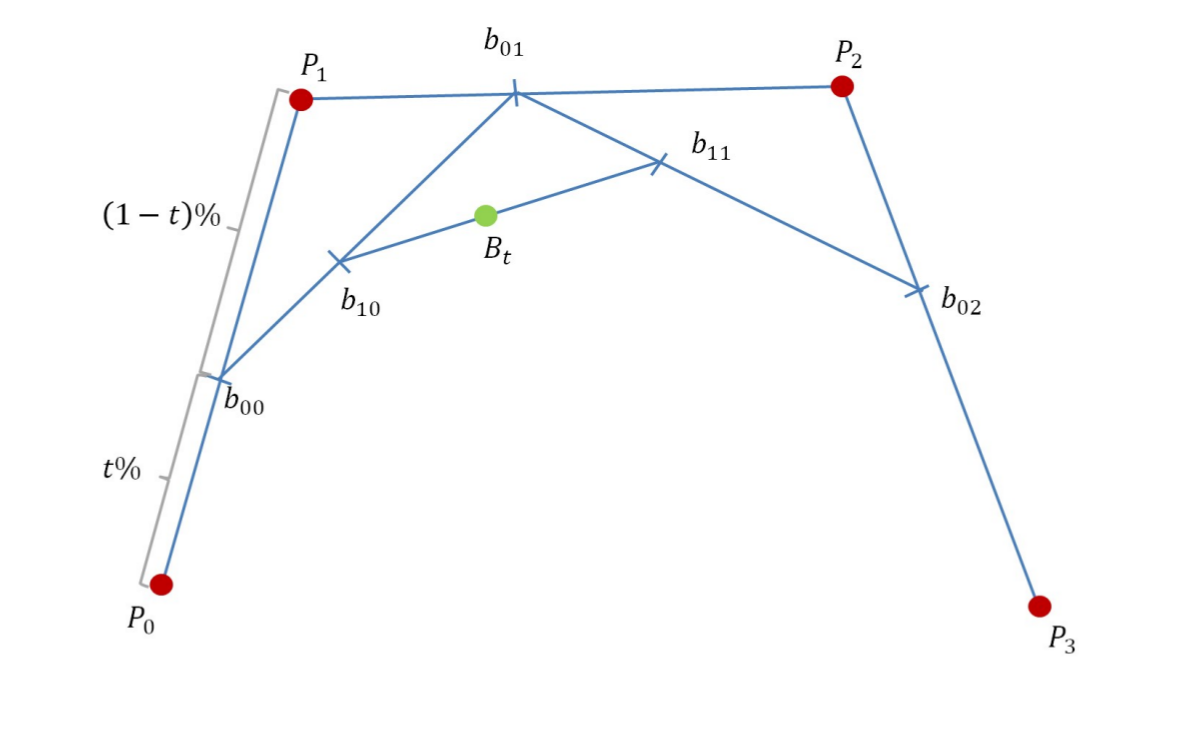
\includegraphics[scale=0.7,keepaspectratio]{resources/casteljou.png}
 	\captionsetup{type=figure, width=0.8\linewidth}
	\caption{Algoritmo geométrico casteljou.png}
\label{fig:ssec1:diagram:plane:to:sphere} 
\end{center}

Fazendo os cálculos manualmente 
\begin{center}
 	
 	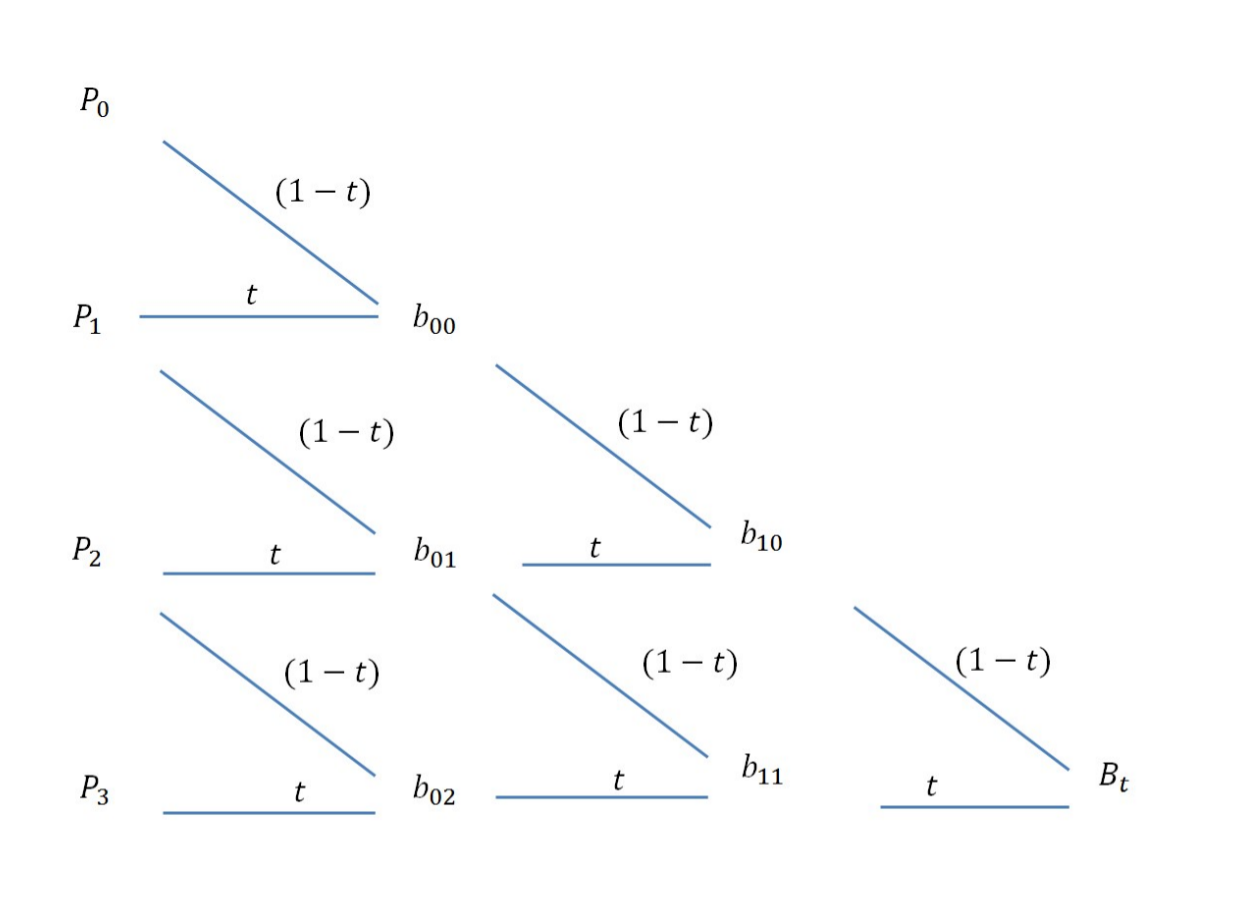
\includegraphics[scale=0.7,keepaspectratio]{resources/casteljeau2.png}
 	\captionsetup{type=figure, width=0.8\linewidth}
	\caption{Representação da árvore casteljeau}
\label{fig:ssec1:diagram:plane:to:sphere} 
\end{center}

Para demonstrar estras tranformações segue-se o exemplo de uma curva de bezier cúbica, isto é, uma curva definida por 4 pontos de controlo:

\begin{center}
 	
 	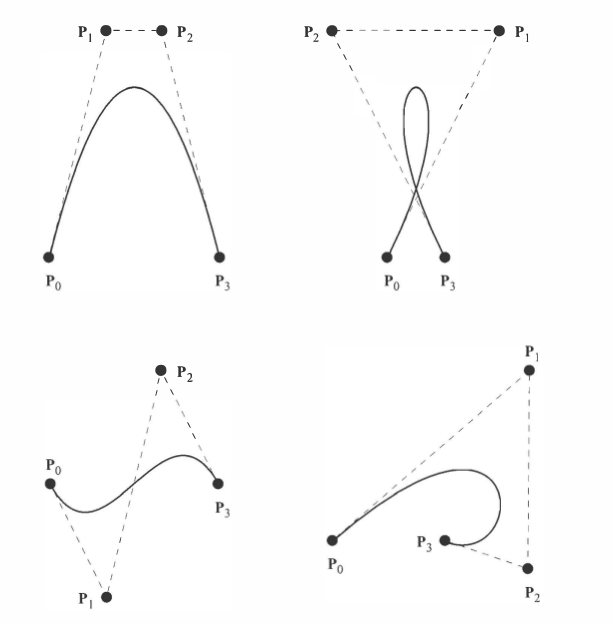
\includegraphics[width=\textwidth,height=\textheight,keepaspectratio]{resources/exemplos1Bezier.png}
 	\captionsetup{type=figure, width=0.8\linewidth}
	\caption{Curvas exemplo de Bezier}
\label{fig:ssec1:diagram:plane:to:sphere} 
\end{center}

Como se pode observar cada uma das curvas observadas possui 4 pontos de controlo, P0, P1, P2 e P3. A figura demonstra alguma das formas que uma curva de Bezier pode tomar. 
As curvas de Bezier, independentemente do número de pontos de controlo que possam ter, são sempre definidas pela seguinte fórmula:
\begin{equation}
B(t)=\sum_{k=0}^{n}B_{n,k}(t)P_{k}
\end{equation}

onde n corresponde a (nº pontos de controlo - 1), e t é o polinómio Bernstein que tem sempre um valor positivo em [0,1] e o seu somatório é sempre igual a 1.




Com 4 pontos de controlo, uma curva de Bezier diz-se cúbica e pode ser definida pela seguinte formula:




\begin{equation}
B(t)=\sum_{k=0}^{3}B_{3,k}(t)P_{k}
\end{equation}

\begin{equation}
B(t)=t^{3}P_{3}+3t^{2}(1-t)P_{2}+3(t(1-t)^{2})P_{1}+(1-t)^{3}P_{0}
\end{equation}

Onde, após cálculos se chegará a:

B(t)=  $\begin{bmatrix}
       t^{3} & t^{2} & t & 1          \\[0.3em]
		\end{bmatrix}$
		$\begin{bmatrix}
		       -1 & 3 & -3  & 1           \\[0.3em]
		        3 & -6 &  3 & 0   \\[0.3em]
		       -3 & 3 & 0 & 0 \\[0.3em]
		       1 & 0 & 0 & 0
		     \end{bmatrix}$
		$\begin{bmatrix}
		       P_{0}           \\[0.3em]
		       P_{1}   \\[0.3em]
		       P_{2} \\[0.3em]
		       P_{3}
		     \end{bmatrix}$


Quanto maior o número de pontos de controlo maior o custo computacional de as representar.

{\huge \textbf{Bezier Patches/superfície:}}

Se se tiver um 2D-array de pontos $P_{i,j}$,i=0,....,m,j=0,....n, então pode-se construir uma superfície bezier da mesma forma que se constrói uma curva Bezier. Da mesma maneira que nas curvas Bezier, a mais importante e mais usada é a superfície de Bezier bicúbica (m=n=3) onde é definida por 16 pontos de controlo $P_{i,j}$ e pode ser escrita da seguite forma:

\begin{equation}
B(u,v)=\sum_{j=0}^{3}\sum_{i=0}^{3}B_{i}(u)P_{i,j}B{j}(v)
\end{equation}



\begin{center}
 	
 	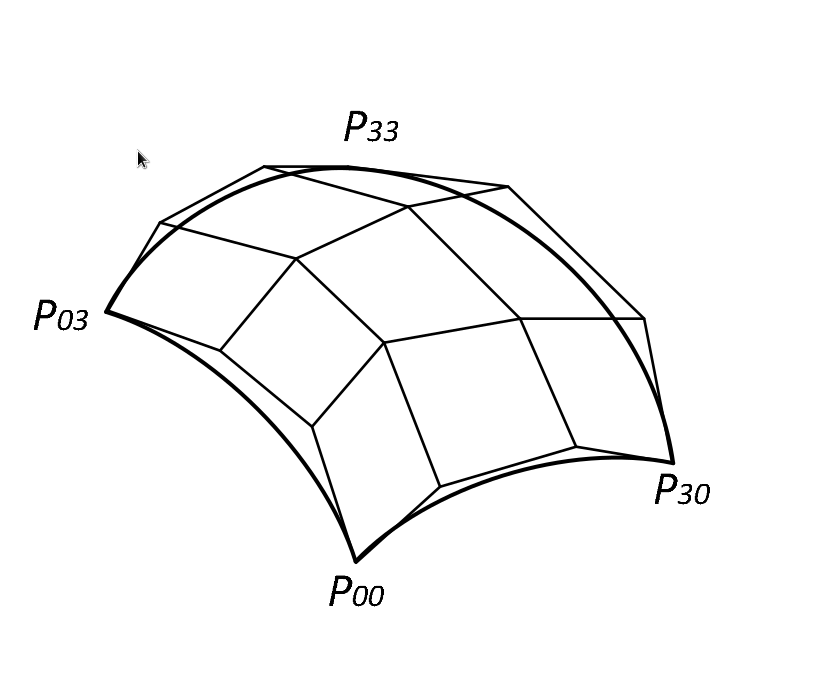
\includegraphics[scale=1,keepaspectratio]{resources/beziersupf.png}
 	\captionsetup{type=figure, width=0.8\linewidth}
	\caption{Superfície de Bezier bicúbica}
\label{fig:ssec1:diagram:plane:to:sphere} 
\end{center}

Sendo U = $\begin{bmatrix}
       u^{3} & u^{2} & u & 1          \\[0.3em]
		\end{bmatrix}$

e M = $\begin{bmatrix}
		       -1 & 3 & -3  & 1           \\[0.3em]
		        3 & -6 &  3 & 0   \\[0.3em]
		       -3 & 3 & 0 & 0 \\[0.3em]
		       1 & 0 & 0 & 0
		     \end{bmatrix}$

Com que foi previamente explicado relativamente às curvas de Bezier, conclui-se que o método de construção de uma superficie Bezier corresponde a um conjuntos de curvas de Bezier conjuntas. 
Então:

B(u,v) = $\begin{bmatrix}
       u^{3} & u^{2} & u & 1          \\[0.3em]
		\end{bmatrix}$ 
		M$\begin{bmatrix}
		       P_{00} & P_{01} & P_{02} & P_{03}   \\[0.3em]
		       P_{10} & P_{11} & P_{12} & P_{13}   \\[0.3em]
		       P_{20} & P_{21} & P_{22} & P_{23}   \\[0.3em]
		       P_{30} & P_{31} & P_{32} & P_{33}
		     \end{bmatrix}$
		$M^{T} \begin{bmatrix}
		       v^{3}           \\[0.3em]
		       v^{2}   \\[0.3em]
		       v^{1} \\[0.3em]
		       v^{0}
		     \end{bmatrix}$

Este método exato irá ser aplicado mais tarde nos algoritmos.
\clearpage

\section{Splines Catmull-Rom}

A curva de splines Catumull-Rom para dados pontos de controlo $P_{0}, P_{1}, P_{2} e P_{3}$, está definida de modo a que a tangente em cada ponto $P_{i}$ possa ser encontrada através da diferença entre os seus pontos vizinhos $P_{i-1}$ e $P_{i+1}$

\begin{center}
 	
 	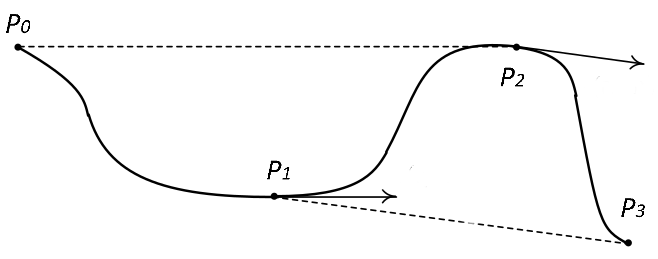
\includegraphics[scale=0.5,keepaspectratio]{resources/catmullDeriv.png}
 	\captionsetup{type=figure, width=0.8\linewidth}
	\caption{Spline Catmull-Rom para os pontos $P_{0}, P_{1}, P_{2} e P_{3}$}
\label{fig:ssec1:diagram:plane:to:sphere} 
\end{center}

Esta curva spline pode ser escrita em forma de matriz:

\begin{equation}
\frac{P_{2}-P_{0}}{2} = P_{1}^{'} = P^{'}(0) = c  \nonumber
\end{equation}
\begin{equation}
P_{1} = P(0) = d 		\nonumber
\end{equation}
\begin{equation}
P_{2}=P(1)=a+b+c+d 		\nonumber
\end{equation}
\begin{equation}
\frac{P_{3}-P_{1}}{2} = P_{2}^{'} = P^{'}(1) = 3a+2b+c 
\end{equation}


o que é equivalante a:

\begin{equation}
P_{0} = a+b-c+d 		\nonumber
\end{equation}
\begin{equation}
P_{1} = P{0} = d 		\nonumber
\end{equation}
\begin{equation}
P_{2}=P(1)=a+b+c+d 		\nonumber
\end{equation}
\begin{equation}
P_{3}=6a+4b+2c+1
\end{equation}

este conjunto de equações pode-se representar na seguinte operação de matrizes:

P=$\begin{bmatrix}
		       P_{0}           \\[0.3em]
		       P_{1}   \\[0.3em]
		       P_{2} \\[0.3em]
		       P_{3}
		     \end{bmatrix}$ = $\begin{bmatrix}
		      					 1 & 1 & -1 & 1           \\[0.3em]
		       					 0 & 0 & 0 & 1   \\[0.3em]
		       					 1 & 1 & 1 & 1 \\[0.3em]
		      					 6 & 4 & 2 & 1
		     					\end{bmatrix}$  $\begin{bmatrix}
		       									a_{x} & a_{y} & a_{z}    \\[0.3em]
		     								  	b_{x} & b_{y} & b_{z}    \\[0.3em]
		       									c_{x} & c_{y} & c_{z}    \\[0.3em]
		       									d_{x} & d_{y} & d_{z} 
		     					\end{bmatrix}$   = $C * A$

Estes cálculos até agora demonstrados irão ser aplicados algoritmicamente no programa da seguinte maneira:

$\begin{bmatrix}
       x(u) & y(u) & z(u)           \\[0.3em]
\end{bmatrix}$ = 
$\begin{bmatrix}
       t^{3} & t^{2} & t & 1          \\[0.3em]
		\end{bmatrix}$ $\begin{bmatrix}
		      					 -0.5 & 1.5 & -1.5 & 0.5           \\[0.3em]
		       					 1 & -2.5 & 2 & -0.5   \\[0.3em]
		       					 -0.5 & 0 & 0.5 & 0 \\[0.3em]
		      					 0 & 1 & 0 & 0
		     					\end{bmatrix}$ $\begin{bmatrix}
         							    P_{0}           \\[0.3em]
       									P_{1}   \\[0.3em]
       									P_{2} \\[0.3em]
       									P_{3}
     \end{bmatrix}$
\clearpage


%---------------------------------------------------------------------------------------------------------------%
\section*{Conclusão\markboth{\MakeUppercase{Conclusão}}{}}
\addcontentsline{toc}{section}{Conclusão}
\label{concl}

Em suma, podemos concluir que o projeto foi um sucesso parcial, dado que não foi
possível iluminar os topos do bule, e que possivelmente poderiam ter sido
efetuados mais testes. Não foram geradas coordenadas de textura para a caixa,
cone e plano, nem vetores normais destas geometrias. No entanto, ficaram
implementadas os vários tipos de luzes, com as suas propriedades de cor, bem
como as propriedades materiais da geometria, assim como a aplicação de texturas.


Como trabalho futuro, sugere-se implementar o cálculo dos vetores normais
e coordenadas de textura para as geometrias que faltam, bem tentar o cálculo de
vetores normais através de interpolação para o bule, tentando diminuir o tamanho
de cada triângulo, para introduzir o efeito MACH ou usar diretamente o modelo
\emph{flat} sabendo das desvantagens de quaisquer um destes métodos. 



\clearpage
% ----------- %
%\bibauthoryear
\nocite{*}
\bibliography{references}
\bibliographystyle{IEEEtran}
%\bibliographystyle{ieeetr}
\clearpage
%%%%%%%%%%%%%%%%%%%%%%%%%%%%%%%%%%%%%%%%%%%%



\appendix 

%\part*{ANEXOS}
%\addcontentsline{toc}{section}{ANEXOS}
\appendix

\part*{ANEXOS}
\addcontentsline{toc}{part}{ANEXOS}
\refstepcounter{part} 

\section{Modelo do Sistema Solar}
\label{appendix:a}
\begin{longlisting}
	\inputminted{xml}{resources/sistema.xml}
	\caption{Código XML com parãmetros para o sistema solar}
\label{listing:b}
\end{longlisting}


\end{document}

%%%%%%%%%%%%%%%%%%%%%%%%%%%%%%%%%%%%%%%%%%%%
